\chapter{Potential outcome model}
\label{chapt:PotentialOM}
The potential outcome model defines the causal effect of an event A as the difference between the two possible states of the world, namely the world where A occurs and the one where A does not occur.
For example, we would like to understand if a medicine can truly improve headaches. Let's formalize the problem by setting X as the set of patient covariates (Age , Gender,... ), D as the treatment regimen (set equal to 1 if the patient takes the medicine and 0 if he takes the placebo), and $Y$ as the number of minutes the headache persists.
Under this model the causal effect of the medicine would be calculated by comparing $Y^{1}_i$ (the world where is administered the medicine), and  $Y^{0}_i$ (the world where the patient is given a placebo). These are the so called "potential outcome" because they are both \textit{a priori} observable, but only one can be observed \textit{a posteriori}. Let's introduce a numerical example, where we somehow know both potential outcomes:
\begin{table}[H]
\centering
\begin{tabular}{|c|c|c|c|c|}
\hline
Age & Sex & $Y^{0}_i$ & $Y^{1}_i$ & $\delta_i$ \\ \hline
20 & M & 20 & 21 & -1  \\ \hline
20 & F & 15 & 3 & 12 \\ \hline
20 & M & 8 & 10 & -2 \\ \hline
20 & F & 16 & 15 & 1 \\ \hline
30 & M & 12 & 13 & -1 \\ \hline
30 & F & 8 & 5 & 3 \\ \hline
30 & M & 2 & 11 & -9  \\ \hline
30 & F & 15 & 26 & 11 \\ \hline
\end{tabular}
\caption{Random trial knowing both potential outcomes }
\label{rt_kbpo}
\end{table}
We can observe that $\delta$ isn't always positive, so the medicine didn't universally improve the situation, but it is seemingly clear that it had positive effects on the whole. This isn't nearly precise enough so we need to introduce some mathematical definitions :
\paragraph{Parameter definition} \hspace{0pt} \\
\label{parag:param}
\begin{itemize}
\item CATE or Conditional Average Treatment Effect is defined as $E[Y^{1}_i- Y^{0}_i|X] = E[\delta_i|X]$, so $CATE_{(M,20)}=E[\delta_i|X=(M,20)] \approx \frac{18-2}{2}=8$ , we can say that on average the medicine caused a reduction of 8 minutes in the length of the headache between 20 year old males.
\item ATE or Average Treatment Effect is defined as  $E[Y^{1}_i- Y^{0}_i] = E[\delta_i]$, so $ATE= E[\delta_i] \approx \frac{18+12-2+18+3-9+11}{8}$.
\item ATT o Average Treatment on the Treated is defined as  $E[Y^{1}_i- Y^{0}_i|D=1] = E[\delta_i|D=1]$ 
\item ATU o Average Treatment on the Untreated is defined as
$E[Y^{1}_i- Y^{0}_i|D=1] = E[\delta_i|D=1]$
\end{itemize}
In this example we somehow know both potential outcomes so we can't calculate the last two quantities.
It is useful to make a distinction between \textit{factual} and \textit{counter factual} values, the former refers to the state of the world we are currently in and the latter refers to \textit{what would have been} if the treatment were different.
We can better understand the distinction between the two through the switching equation: 
\begin{equation}
Y_i^{obs} = D_i \cdot Y^1_i + (1-D_i) \cdot Y^0_i
\label{eq:switching}
\end{equation}
We can see that $Y^1_i$ is either a \textit{factual} value when $D_i=1$ or \textit{counter factual} when $D_i=0$.
It's obvious that in a real setting, we wont ever be able to fill in all the data like in table \ref{rt_kbpo}, at least half of the value will be missing.
An example of such table could be the following:
\begin{table}[H]
\centering
\begin{tabular}{|c|c|c|c|}
\hline
Age & Sex & $Y^{0}_i$ & $Y^{1}_i$ \\ \hline
20 & M & 20 & ?  \\ \hline
20 & F & 15 & ? \\ \hline
20 & M & ? & 10 \\ \hline
20 & F & ? & 15  \\ \hline
30 & M & 12 & ? \\ \hline
30 & F & 8 & ? \\ \hline
30 & M & ? & 11   \\ \hline
30 & F & ? & 26 \\ \hline
\end{tabular}
\caption{Table random trial}
\end{table}
The potential outcome model manages to transform the intractable problem of causation in to a much more manageable problem of \textit{missing data}.

\section{Assumptions and exclusion restriction}
So far we hid a few of the assumption to avoid making this introduction unnecessary cumbersome however it is now necessary to point them out to avoid confusion.
These are the so called \textit{exclusion  restriction} : assumption made with substantive knowledge of the subject matter. In fact any of these assumptions can be loosened if the specific case requires it, but they are considered to be the most common assumption when tackling a problem of causal inference \citep{imbens2015causal}.
This \textit{exclusion restriction} first proposed in  \citep{rubin1980randomization}, states that :
\begin{ass}{SUTVA}
The potential outcome for any unit do not vary with the treatments assigned to other units and, for each unit, there are no different forms or versions of each treatment level, which lead to different potential outcomes.
\label{sutva}
\end{ass}
\citep{imbens2015causal}
This assumption can be split in two parts, the no interference component and the no hidden variation of treatment components. The former implies that any potential outcomes for a given observation are independent from treatment of other units, it can be expressed by :
$$ D_j \perp\!\!\!\perp (Y^{0}_i,Y^{1}_i) \ \forall i \not = j $$ [to check if the mathematical expression is true]
For example in the headache situation we excluded \textit{a priori} that each unit treatment wouldn't effect other patients, of course this kind of assumption ought to be carefully considered  by an expert on a case by case basis.
However this assumption becomes shaky when we consider time series or pandemics where a unit treatments is very likely to impact the other units. The problem can be solved in two ways either by having a more suiting \textit{exclusion restriction} or by defining a unit in a broader term, in the vaccination example the unit could be the nation (given no spillover between nations), instead of the individual. 
The second component instead implies that the treatment is homogeneous in the population, so back to the headache example we cannot have a medicine that has different potency or is administered in different ways.
This assumption referred to a DAG states the arrow from treatment D to outcome Y corresponds to unambiguous and uniform intervention. 
The assumption of strong ignorability was first formalized in \citep{rosenbaum1983central} , and aims to restrict the possible assignment mechanism  (should i define a assignment mechanism ?) and has three main components :
\begin{ass}[Individualistic assignment]
An assignment mechanism is individualistic if $Pr(D_i| X_i , Y_i^0 ,Y_i^1) = q( X_i , Y_i^0 ,Y_i^1)$ for some function $q(.)$
\end{ass}{Strong ignorability}
This means that weather a unit gets a treatment its a function only of its own covariates.
\begin{ass}[Probabilistic assignment]
An assignment mechanism is probabilistic if $Pr(D_i| X_i , Y_i^0 ,Y_i^1)$ is bounded strictly between 0 and 1 $\forall X,Y^1,Y^0,i$
\end{ass}
This requirement is important because we need to see the counter factual in the limit of all possible subpopulations. The estimation if this condition is not met, is practically impossible, because it means that we don't have any data about how a subset of the population would react to treatment, thereby any causal estimation would rely only on extrapolation.  In the causal DAGs  drawn so far, probabilistic assignment is implicit, and SUTVA is embedded in the notation because we only consider treatment nodes with binary and well defined alternatives. Probabilistic assignment is concerned with arrows going into the treatment nodes, and SUTVA is only concerned with arrows leaving the treatment nodes.
Thus, the treatment nodes are implicitly given a different status compared with all other nodes.\citep{hernan2020causal}
\begin{ass}[Unconfounded assignment]
An assignment mechanism $Pr(D_i| X_i , Y_i^0 ,Y_i^1)$ is unfounded if  it does not depend on the potential outcomes $Pr(D_i| X_i , Y_i^0 ,Y_i^1)= Pr(D_i| X_i )$ or $D_i  \perp\!\!\!\perp (Y^{0},Y^{1}) | X$
\end{ass}
\label{ass:Unconfounded assignment}
This means that once conditioned on the set of variables ${X}$ , having information on $Y$ doesn't give us further information about the treatment status. The independence above might remind the reader of the consequence of having satisfied the backdoor criterium, in fact once we have a conditioning set ${X}$ that satisfies it, this implies that the unconfounded assignment holds \citep{cunningham2021causal}. The contrary is also true, unconfounded assignment and faithfulness imply that the backdoor criterium is satisfied. \citep{hernan2020causal}
\\
this assumption is not testable (pag 261 IR) [should i add something about this ]
%pag 38-39 rubin imbens
% individualistic treatment see if it is meaningfully different from SUTVA
% uncofoundeness (satifies back door criterion)
% probabilistic treatment
%dawid 1979
%"fan li : a tutorial on causal inference"
%\subsection{Superpopulation and finite samples}
%From now on we will make another type of distinction between whether our interest is related to the finite sample  or to larger \textit{superpopulation} where the finite sample is drawn from  [riguardare] 
\section{Randomized studies}
We often hear about double-blind randomized trials, that is where some of the patients are given the medicine and the other are given a placebo with neither the doctors nor the patients being aware of who received what. Such trial can be expressed through a DAG in this way: 
\begin{figure}[H]
\centering
	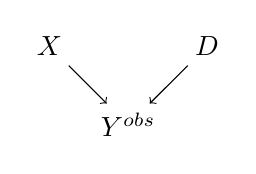
\begin{tikzpicture}
		\node (x) at (0,1) {$X$};
    		%\node (yz) at (0,0) {$Y^{1}$};
    		%\node (yo) at (2,0) {$Y^{0}$};
		\node (y) at (1,0) {$Y^{obs}$};
    		\node (D) at (2,1) {$D$};
    		%\path[->] (x) edge (yz);
    		%\path[->] (x) edge (yo);
    		\path[->] (x) edge (y);
    		%\path[<-] (T) edge (x);
    		\path[->] (D) edge (y);
	\end{tikzpicture}
\caption{Dag for randomized trial}
\label{fig:dag_random_EX}
\end{figure}
Why is this kind of trial become the golden standard for causal inference? What can such a trial truly tell us?
Under the potential outcome model this kind of trial imply this independence:
\begin{equation}
D \perp\!\!\!\perp (Y^{0},Y^{1})
\end{equation}
\label{eq:indipendence_r}
Of course this independence is stronger than the assumption \ref{ass:Unconfounded assignment}, because we don't have to condition upon X; this is a natural consequence of the assignment mechanism being blind to covariates $$Pr(D_i| X_i , Y_i^0 ,Y_i^1) = c $$ 
This also means that the potential outcomes didn't play a role in determining the treatment regime. However it \textbf{doesn't} imply that $D \perp\!\!\!\perp Y^{obs}$, in fact is patently false each time a medicine has an effect on a patient. By virtue of equation \ref{eq:indipendence_r}, we can state that $E[Y^1_i] = E[Y^{1}_i | D_i = 1]  $ and the same for $E[Y^0_i] = E[Y^{0}_i | D_i = 0] $.
We can assert that:
\begin{align}
ATE &= E[Y^1_i-Y^0_i ] \\ 
 &= E[Y^{1}_i | D_i = 1]- E[Y^{0}_i | D_i = 0]\label{eq:ATE_R} \\
	& =E[Y^{1}_i | D_i = 1]- E[Y^{0}_i | D_i = 1] \label{eq:ATT_R} \\
 &= E[Y^{1}_i | D_i = 0]- E[Y^{0}_i | D_i = 0]. \label{eq:ATU_R}
  \end{align}
In the equation \ref{eq:ATE_R} both quantities are \textit{factual}, through the law of large number we can estimate both as means. We will define as SDO the simple difference in group means in the finite sample:
$$SDO := \frac{1}{N_1}\sum_{i:d_i=1}y_i - \frac{1}{N_2}\sum_{i:d_i=0}y_i \overset{\underset{\mathrm{(N_1, N_2) \rightarrow \infty}}{}}{=} ATE.$$
We can also conclude from equation \ref{eq:ATT_R} and \ref{eq:ATU_R} that in a randomized trial  $ATE = ATT = ATU$.
\subsection{Parte empirica}
% crucial to understand the difference bewteen definition and estimation 
\section{Observational studies} % esiste il termine?
Observational studies are much different; researchers gather data that isn't intended to be randomized trials, were the researchers cannot intervene and impose the randomization, for two main reason :
\begin{enumerate}
\item Ethical or practicability concerns  (e.g.: if we wanted to know whether smoking causes cancer)
\item The events might have already taken place  (e.g.: if we wanted to study the effect of a certain policy)
\end{enumerate}
The main difference is that $D \not \perp\!\!\!\perp (Y^{0},Y^{1})$, we can represent this too with a DAG:
\begin{figure}[!h]
\centering
	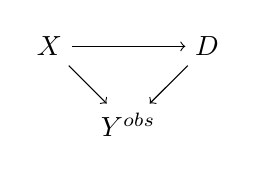
\begin{tikzpicture}
		\node (x) at (0,1) {$X$};
    		%\node (yz) at (0,0) {$Y^{1}$};
    		%\node (yo) at (2,0) {$Y^{0}$};
    		\node (y) at (1,0) {$Y^{obs}$};
    		\node (D) at (2,1) {$D$};
    		%\path[->] (x) edge (yz);
    		%\path[->] (x) edge (yo);
    		\path[->] (x) edge (D);
    		\path[->] (x) edge (y);
    		\path[->] (D) edge (y);
    		%\path[<-] (T) edge (x);
    		%\path[->] (T) edge (y);
	\end{tikzpicture}
\caption{Dag per studio osservazionale}
\label{fig:dag_OBS}
\end{figure} \\
if exchengiabilty holds \ \
matching (exact and not ) \\
prop score IPW \\ 
this part has to be flushed out more fully.








